% interactapasample.tex
% v1.05 - August 2017

\documentclass[]{interact}

\usepackage{epstopdf}% To incorporate .eps illustrations using PDFLaTeX, etc.
\usepackage[caption=false]{subfig}% Support for small, `sub' figures and tables
%\usepackage[nolists,tablesfirst]{endfloat}% To `separate' figures and tables from text if required
%\usepackage[doublespacing]{setspace}% To produce a `double spaced' document if required
%\setlength\parindent{24pt}% To increase paragraph indentation when line spacing is doubled

%\usepackage[longnamesfirst,sort]{natbib}% Citation support using natbib.sty
%\bibpunct[, ]{(}{)}{;}{a}{,}{,}% Citation support using natbib.sty
%\renewcommand\bibfont{\fontsize{10}{12}\selectfont}% To set the list of references in 10 point font using natbib.sty
\usepackage[natbibapa,nodoi]{apacite}
\setlength\bibhang{12pt}
\renewcommand\bibliographytypesize{\fontsize{10}{12}\selectfont}

\usepackage{lmodern}
\usepackage{bbm,bm}
\usepackage{amssymb,amsmath,longtable,bm,multirow}
\usepackage{ifxetex,ifluatex,booktabs}
\usepackage{fixltx2e} % provides \textsubscript
\usepackage{amsmath, mathtools, amsfonts}
\usepackage{fancyhdr, geometry}
\usepackage{lastpage}
\usepackage{pgfplots,pgf}
\usepackage{tikz}
\usepackage{float}
\usepackage{algorithm}
\usepackage{algpseudocode,indentfirst}
\usepackage{color,listings}
\usepackage{hyperref}
\hypersetup{unicode=true,
            pdftitle={Knockoff Adjusted P-Values},
            pdfborder={0 0 0},
            breaklinks=true}
            
%\usepackage[natbibapa,nodoi]{apacite}% Citation support using apacite.sty. Commands using natbib.sty MUST be deactivated first!
%\setlength\bibhang{12pt}% To set the indentation in the list of references using apacite.sty. Commands using natbib.sty MUST be deactivated first!
%\renewcommand\bibliographytypesize{\fontsize{10}{12}\selectfont}% To set the list of references in 10 point font using apacite.sty. Commands using natbib.sty MUST be deactivated first!

\theoremstyle{plain}% Theorem-like structures provided by amsthm.sty
\newtheorem{theorem}{Theorem}[section]
\newtheorem{lemma}[theorem]{Lemma}
\newtheorem{corollary}[theorem]{Corollary}
\newtheorem{proposition}[theorem]{Proposition}

\theoremstyle{definition}
\newtheorem{definition}[theorem]{Definition}
\newtheorem{example}[theorem]{Example}

\theoremstyle{remark}
\newtheorem{remark}{Remark}
\newtheorem{notation}{Notation}

\newcommand{\E}{\mathrm{E}}
\newcommand{\Var}{\mathrm{Var}}
\newcommand{\Cov}{\mathrm{Cov}}
\newcommand{\prob}{\mathrm{Pr}}
\providecommand{\tightlist}{%
  \setlength{\itemsep}{0pt}\setlength{\parskip}{0pt}}
\begin{document}

%\articletype{ARTICLE TEMPLATE}% Specify the article type or omit as appropriate

\title{Knockoff Procedure for False Discovery Rate Control in High-Dimensional Data Streams}

\author{
\name{Ka Wai Tsang\textsuperscript{a}, Fugee Tsung\textsuperscript{b}, and Zhihao Xu\textsuperscript{c}}
\affil{\textsuperscript{a,c}School of Data Science, The Chinese University of Hong Kong, Shenzhen; \textsuperscript{b} Department of Industrial Engineering and Decision Analytics, Hong Kong University of Science and Technology, Hong Kong}
}

\maketitle

\begin{abstract}
Motivated by applications to root-cause identification of faults in high-dimensional data streams that may have very limited samples after faults are detected, we consider multiple testing in models for multivariate statistical process control. With quick fault detection, only small portion of data streams being out-of-control (OC) can be assumed. It is a long standing problem to identify those OC data streams while controlling the number of false discoveries. It is challenging due to the limited number of OC samples after the termination of the process when faults are detected. We propose a knockoff procedure to control the false discovery rate (FDR). The theorem for the FDR control of the knockoff procedure without the requirement of large sample size is provided. Simulation and empirical studies show that the proposed procedure can control FDR while maintain high power. We also illustrate the performance in an application to semiconductor manufacturing processes that motivated this development.
 
\end{abstract}

\begin{keywords}
Fault identification; Multiple testing; Statistical process control; Multistage manufacturing process; Knockoff filtering.
\end{keywords}

\section{Introduction}\label{introduction}

Nowadays, high-dimensional data streams can be easily obtained in modern manufacturing and service industries. Together with the increasing low computational cost to handle big data, people are more willing to use high-dimensional data streams to build statistical models for monitoring complex systems and quality control. It makes the conventional tools for multivariate statistical process control (SPC) become difficult and even impossible, to apply in practice. The tasks of multivariate SPC basically include fault detection, which determines if there exist changes in the data streams, and fault identification, which isolating the components that are responsible for the changes. Beginning with acceptance sampling and Shewhart’s control charts that use relatively simple univariate quality characteristics, multivariate quality control characteristics and more efficient SPC schemes such as multiple cumulative sum (CUSUM) and exponentially weighted moving average (EWMA) have been developed and commonly used due to the advances in multivariate analysis and sequential analysis in the statistical literature. Because of the availability of “big data” for fault detection and identification and recent developments in the statistics literature on high-dimensional data analysis, the analysis for multivariate SPC has moved to a new direction in the past decade. For fault detection, the recent development for high-dimensional data streams can be found in \cite{woodall2014some}, \cite{zou2015efficient}, \cite{xian2018nonparametric}. While many diagnostic procedures have been proposed for fault detection and identification, most of them do not guaranteed to control false alarm rate, which may result in resource wasting on false alarms, or require sufficient OC samples generated for fault diagnosis after a fault alarm is detected, which may not be possible in practice. In this paper, we introduce a novel knock-off procedure for fault identification for high-dimensional data streams that can control FDR even if the number of OC samples is small.


Suppose we observe independent $X_{j,t}$ for the $j^{th}$ data stream at time $t = 1, 2, \ldots $ for $j = 1, \ldots, m$, with the number of streams being $m$. After a change-point $v$, the distributions of the observations from some proportion of the streams get changed. Hence for the $j^{th}$ data stream, the density function of $X_{j,t}$ is $f_0^{j}$ for $t<v$, and is $f_1^j$ for $t \ge v $. This leads to the null hypothesis 
\begin{align}
H_j: f_1^j = f_0^j,\quad j=1,\ldots,p, \label{p Hj}
\end{align}
or equivalently, the $j^{th}$ data stream is not among those data streams that change their distributions at the change point $v$. Let $\mathbf{X}_t = [X_{1,t}, \ldots, X_{m,t}]^T$, $\bm{\mu}_0 = \E(\mathbf{X}_t)$ for $t<v$ and $\bm{\mu} = \E(\mathbf{X}_t)$ for $t\ge v$. We assume the covariance matrix $\bm{\Sigma} = \Var(\mathbf{X}_t)$ remains the same for all $t$ and there is mean shift for the $j^{th}$ stream if $f_1^j \ne f_0^j$. Therefore, assume $\bm{\mu}_0$ is a zero vector, our hypotheses are $H_{j}: \mu_{j} = 0$ versus $H_{j}^A: \mu_{j} \ne 0$ for $j = 1, \ldots, m$ where $\mu_j$ is the mean of $f_1^j$. When $m$ is small, a common test statistic used for fault detection and identification is Hotelling's $T^2$. To locate the mean shifts, different decompositions of Hotelling's $T^2$ statistics have been developed (\cite{mason1995decomposition}, \cite{mason1997practical}, \cite{li2008causation}). \cite{zhu2009adaptive} points out that such decomposition ''depends on a prespecified order of variables and known a priori''. As the shift structures may not be known in practices, \cite{zhu2009adaptive} propose an adaptive $T^2$ chart, which does not require a priori knowledge of the potential shifts space, for fault detection and identification. However, when $n$ is large, \cite{li2020diagnostic} comment that 	``the decomposition of the $T^2$ statistic consider $m!$ different decompositions of the $T^2$ statistic, and the standard step-down testing procedures still require the computation of $\binom{m}{k}$ test statistics of quadratic-term in the $k^{th}$ step'' and point out that ``both methods are very time consuming.'' Another issue for multivariate SPC to the high dimensionality is the signals of those shifted streams, or OC streams, can be buried in the large amount of unshifted streams, or in-control (IC) streams, and thus become difficult to detect. \cite{wang2009high} illustrate this issue by showing the detection power of a Hotelling's $T^2$ chart with dimension $m$ and one shifted stream. They show that the shift can be detected with very high probability $(0.982)$ when $n=1$, but the detection probability drops to $0.018$ when the dimension $m$ increases from $1$ to $20$.

To handle the high dimensionality, various methods based on variable selection have been proposed recently. \cite{wang2009high} consider a penalized optimization problem to find a sparse estimator of $\mu$ such that a linear combination of the generalized distance with the sample mean and a LASSO-type penalty is minimum. \cite{liang2016robust} extend their ideas of using LASSO penalty to non-normal situations. Instead of LASSO penalty, \cite{jiang2012variable} and \cite{li2017robust} consider Lo penalty of the $\Sigma_j \mathbbm{1}_{ \{|\mu_j| \ne 0 \}} \le s$ to select $s$ data streams instead of selecting streams by penalized optimization, \cite{mei2011quickest} proposes a top-r thresholding scheme to select $r$ streams with largest local CUSUM statistics. \cite{capizzi2011least} and \cite{ing2017multiple} model the main shifts as linear combinations of some explanatory variables and thus formulate the fault identification problem as variable selection problem in linear regression models. These variable selection methods are designed to select almost all significant signals (mean shifts). However, it is also important for these methods to avoid selecting too many false alarms. Otherwise, many resources will be wasted on checking those false alarms. \cite{ing2017multiple} propose an OGA procedure to control the family-wise error rate (FWER), which is the probability existing false alarms in the selection set. However, since it is usually not a matter to have a few, but not many, false alarms in practice, controlling FWER can be unnecessarily too conservative. Besides, their OGA procedure requires the number of OC observations large enough to asymptotically control FWER, which may not be possible in practice. As \cite{li2020diagnostic} points out that ''In most SPC applications, a major goal is to detect a change as quickly as possible and, if this goal is attained, there may be only a few OC observations collected since the process is always shut down after a signal.'' Therefore, the performance of their OGA procedure can be poor for limited number of OC observation. A less conservative error rate that is commonly considered to control is the false discovery rate (FDR), which is the expected ratio of the false alarms to the number of all of the rejected hypotheses. \cite{li2009false} apply Benjamini and Hochberg's (BH) procedure to establish FDR-adjusted Shewhart chart and FDR-adjusted CUSUM chart. However, their proposed schemes do not guarantee the control of FDR. \cite{du2018line} develop a dynamic multiple testing procedure for high dimensional multivariate SPC with the control of FDR at each time point, but not at the stopping time when signals are detected. These variable selection based schemes are mainly focus on online fault detection, but not fault identification. These methods select a set of data streams at each time point, and then conduct hypotheses testing or check criteria to detect signals. The number or the ratio of false discoveries in the selected set at the stopping time is not guaranteed to be controlled. For controlling FDR after variable selection, recently \cite{barber2015controlling} propose a variable selection procedure, knockoff filtering, that control FDR in the linear regression setting and their empirical results show that knockoff filtering has higher power than other selection methods with FDR controlled at the same level when the proportion of null hypotheses is high. In this paper, we apply their ideas to propose a knockoff procedure for fault identification with the control of FDR.

A brief introduction of knockoff filtering is presented in Section 2, in which we give our general algorithm for fault identification with theoretical justification for the control of FDR. Our general algorithms can be applied with various variable selection methods. Two particular variable selection methods are considered in Sections 3 and 4 to illustrate the use of our general algorithm. In Section 5, we apply our method to fault diagnosis based on a real dataset from a semiconductor manufacturing process. Section 6 gives further discussion of the application of our proposed knockoff procedure.


\section{Knockoff procedure}

\cite{barber2015controlling} introduce a powerful variable selection procedure, called knockoff filtering, controlling the FDR in the statistical linear model whenever there are at least as many observations as hypotheses. They consider the linear model $y_t = \sum_{j=1}^p X_{tj} \beta + \varepsilon_t, t=1,\ldots,n$, where $\varepsilon_t$ are error terms independent of $X_{tj}$ with mean $0$. They are interested in testing $H_j: \beta_j=0$ for $j=1,\ldots, p$ and restrict their attention to the case where $n \ge p$. Such restriction is released in \cite{barber2019knockoff} who have extended knockoff filtering to the high-dimensional setting. The core part of knockoff filtering is the construction of knockoff variables that are defined to be pairwise exchangeable with the originals $\bm X_j = [X_{1j}, \ldots, X_{nj}]^T, j = 1, \ldots, p$, but not related to $\bm y = [y_1, \ldots, y_n]^T$. Let $\bm{\tilde X}_j$ be a knockoff variable for $\bm X_j$, then if $H_j$ is true, the joint distribution of $[\bm X, \bm{\tilde X}] = [\bm X_1, \ldots, \bm X_p, \bm{\tilde X}_1, \ldots, \bm{\tilde X}_p]$ does not change when $\bm X_j$ and $\bm{\tilde X}_j$ are swapped. More generally, for any subset $T$ of the set of null hypotheses $H_0$, swapping columns of $\bm X_j$ and $\bm{\tilde X}_j$ for any $j \in T$ does not change the distribution of $[\bm X, \bm{\tilde X}]$. With such exchangeable knockoff variables, a set of variable importance statistics $[\bm Z, \bm{\tilde Z}] = [Z_1, \ldots, Z_p, \tilde Z_1, \ldots, \tilde Z_p]$, which reflects the importance of $\bm X_j$ and $\bm{\tilde X}_j$, can then be computed. For example, if we apply a forward stepwise selection algorithm, e.g. orthogonal greedy algorithm in \cite{ing2017multiple}, on $[\bm X, \bm{\tilde X}]$ and $\bm y$, then $Z_j (\tilde Z_j)$ can be defined as the order of selection of $\bm X_j (\bm{\tilde X}_j)$. Note that if $H_j$ is true, $\bm X_j$ and $\bm{\tilde X}_j$ are of the same importance. Otherwise, $\bm X_j$ is more likely to be selected before $\bm{\tilde X}_j$ as $\bm{\tilde X}_j$ is not related to $\bm y$, and thus $Z_j$ is expected to be smaller than $\tilde Z_j$ in such case. And then we can construct knockoff statistics $W_j = W(Z_j, \tilde Z_j)$ such that $W_j$ satisfies (i) flip-sign property $W_j = W(Z_j, \tilde Z_j) = -W(\tilde Z_j, Z_j)$ and (ii) if $H_j$ is true, $P(W_j > t) = P(W_j < t)$ for all $t>0$ and $P(W_j > t) > P(W_j < t)$ if $H_j$ does not hold. In the previous forward stepwise example, we can take $W_j = Z_j - \tilde Z_j $. Note that conditioning on $|W_j|$, the signs of the $W_j$'s corresponding to null $H_j$ are distributed as i.i.d. fair coin flips and $W_j$'s are expected to be positive if $H_j$ is that depends on the number of $W_j$'s being positive if $H_j$ is false. It suggests rejecting $H_j$ for those $W_j$ passing same threshold that depends on the number of $W_j$'s being positive and negative. \cite{barber2015controlling} define the knockoff estimate of false discovery proportion (FDP) as
\begin{equation}\label{eq1}
\widehat{FDP}(t) = \frac{1 + \# \{j: W_j \le -t\}}{\max \{1, \#\{j: W_j \ge t\}\}}
\end{equation}
and reject $H_j$ if $W_j \ge t_{\min}$ where $t_{\min} =\min \{t: \widehat{FDP}(t)  \le \alpha\}$ to control the FDR at $\alpha$ level.

For the multivariate SPC problem, suppose we observe $p$ data streams $\bm{X}_{j,\cdot} = [X_{j,1}, \ldots, X_{j,\tau^{obs}}]^T$ after the change-point $v$, which is assumed to be known or can be well estimated by some change-point methods, see, for example, \cite{zamba2006multivariate}. The observed stopping time after $v$ is supposed to be small since the process should be stopped after a signal is detected. We assume $\tau^{obs} = \tau \left( \{X_{j,1}, X_{j,2}, \ldots\}, j=1, \ldots, p \right)$ is a function of a set of data streams. If $X_{j,t}$ with the null density function $f_0^j$ are independent, then we can simply generate a knockoff copy for $\bm X_{j,\cdot}$ by generating $\bm{\tilde X}_{j,\cdot} = [X_{j,1}, \ldots, X_{j,\tau^{obs}}]^T$ from the known density $f_0^j$. Let $\tau^{KF}=\tilde \tau (\{ X_{j,1}, X_{j,2}, \ldots\} \cup \{ \tilde X_{j,1},\tilde X_{j,2},\ldots\}, j=1, \ldots, p)$ be the new stopping time for $p$ original data streams and their knockoff copies. The stopping rule $\tilde \tau$ is chosen such that $\tau^{KF} \le \tau^{obs}$. For example, for top-r procedure, the original stopping time $\tau$ is the sum of largest $r$ CUSUM statistics being greater than or equal to some threshold $a$. In such case, we can choose $\tilde\tau=\tau$ since the sum of largest $r$ CUSUM statistics of the original data streams and knockoff copies must be greater than or equal to $a$. In general, we can select a set of $p$ data streams at each time $t \le \tau^{obs}$ such that the stopping time $\tau$ is most likely to be satisfied, e.g. choosing a set of $p$ data streams with largest absolute sample mean or with largest CUSUM statistics, or with smallest p-value etc. By defining $\tilde \tau$ to be first selecting the $m$ data streams with most significant signals, and then apply $\tau$ on the selected set, we can guarantee $\tau^{KF} \le \tau^{obs}$. For a data stream $X_{j,t}$ with $f_0^j = f_1^j$, i.e. $H_j$ is true, $X_{j,t}$ and the corresponding knockoff copy $\tilde X_{j,t}$ have the same distribution. Therefore, we can compute the corresponding variable importance statistics $Z_j$ and $\tilde Z_j$ (e.g. the sample means of $X_{j,t}$ and $\tilde X_{j,t}, t=1, \ldots, \tau^{KF})$ such that $Z_j$ and $\tilde Z_j$ have the same distribution, and hence the knockoff procedure can be applied to control FDR.

General knockoff procedure for multivariate SPC.
\begin{enumerate}
\tightlist
\item Generate knockoff copies $\tilde X_{j,t}$ of observed $X_{j,t}$ for $j=1, \ldots, p, t = 1, \ldots, \tau^{obs}$
\item Compute the new stopping time $\tau^{KF}=\tilde \tau (\{ X_{j,1}, X_{j,2}, \ldots\} \cup \{ \tilde X_{j,1},\tilde X_{j,2},\ldots\}, j=1, \ldots, p)$. The stopping rule $\tilde \tau$ is chosen such that $\tau^{KF} \le \tau^{obs}$
\item Compute $Z_j = Z_{j,\tau^{KF}}$ and $\tilde Z_j =\tilde Z_{j,\tau^{KF}}$, where
$$
Z_{j,t} = \max \left \{Z_{j,t-1} + X_{j,t}, 0 \right \} \text{  and  } \tilde Z_{j,t} = \max \left \{\tilde Z_{j,t-1} + \tilde X_{j,t}, 0 \right \}
$$
with $Z_{j,0} = \tilde Z_{j,0} = 0$. Set $W_j=Z_j - \tilde Z_j$ for $j=1, \ldots, p$.
\item Reject $H_j$ if $W_j \ge t_{\min}$ where $t_{\min} = \min \{t : \widehat{FDP}(t) \le \alpha\}$.
 \end{enumerate}

Here we consider CUSUM chart for computing $Z_j$ and $\tilde Z_j$ in Step 3 as it has been proven optimal properties for a given size of mean shift, see \cite{bagshaw1975influence}.

If $\bm X_{j,\cdot} = [X_{j,1}, \ldots, X_{j,\tau^{obs}}]^T$ are independent, $\bm{\tilde X}_{j,\cdot} = [\tilde X_{j,1}, \ldots, \tilde X_{j,\tau^{obs}}]^T$ in Step 1 can be generated by the known density $f_0^j$. If not, the correlation among $\bm X_1, \ldots, \bm X_p$ needs to be considered in the construction of knockoff copies to ensure that the distributions of $\bm X_j$ and $\bm{\tilde X}_j$ are the same. If $\bm X_{j,\cdot}, j=1,\ldots,p$, are not independent, we further assume that $f^j_0$ is the density function of $\mathcal{N} (0,1)$, the density $f_1^j$ after the change-point $v$ is the density function of $\mathcal{N} (\mu_j, 1)$, and the joint density of $\bm X_{\cdot, t} = [X_{1,t}, \ldots, X_{p,t}]^T$ after $v$ is $\mathcal{N} (\bm \mu, \bm \Sigma)$. In such case, we follow the ideas in \cite{barber2015controlling} to construct $\bm{\tilde X}_{\cdot, t} = [\tilde X_{1,t}, \ldots, \tilde X_{p,t}]^T$ that follows 
\begin{equation} \label{eq2}
\begin{bmatrix}
\bm X_{\cdot,t} \\
\bm{\tilde X }_{\cdot,t}
\end{bmatrix}
\sim
N \left ( 
\begin{bmatrix}
\bm \mu \\
\bm 0
\end{bmatrix},
\begin{bmatrix} 
\bm \Sigma & \bm \Sigma - diag(\bm s) \\ 
\bm \Sigma - diag(\bm s) & \bm \Sigma 
\end{bmatrix}
\right),
\end{equation}
where $\bm s = [s_1, \ldots, s_p]$ is chosen such that the covariance matrix in (\ref{eq2}) is positive semi-definite. Equivalently, for each $t$ with given observation $\bm X_{\cdot, t}$, $\bm{\tilde X}_{\cdot, t}$ can be generated from the conditional distribution
\begin{equation}\label{eq3}
\bm{\tilde X}_{\cdot, t}|\bm X_{\cdot, t} \sim \mathcal{N}\left((\bm \Sigma - diag(\bm s))\bm \Sigma^{-1} (\bm X_{\cdot,t} - \bm \mu), \bm \Sigma - (\bm \Sigma-diag(\bm s))\bm \Sigma^{-1}(\bm \Sigma-diag(\bm s)\right)
\end{equation}
\cite{barber2015controlling} show that the generated knockoff copies $\bm{\tilde X}_{j, \cdot}$ satisfy the pairwise exchangeable property with $\bm X_{j, \cdot}$. For the choice of $\bm s$, we simply consider $s_j = \min \left(1, 2 \lambda_{\min}(\bm \Sigma)\right)$ for all $j$, which is suggested in \cite{barber2015controlling}. Another suggested choice is to choose $\bm s$ such that the average correlation between $X_{j,t}$ and $\tilde X_{j,t}$ is minimum for higher power. It can be constructed by minimizing $\sum_{j=1}^p |1 - s_j|$ with the constraints $s_j \ge 0$ and $2 \bm \Sigma - diag(\bm s)$ is positive semi-definite. In practice, the mean shift $\bm \mu$ is unknown and hence we can only use an estimate $\bm{\hat \mu}$ to replace $\bm \mu$ in the $\bm{\tilde X}_{\cdot,t}$ generation equation (\ref{eq3}). An intuitive choice of $\mu_j$ estimate is the sample mean $\bm{\hat \mu} = \sum_{t=1}^{\tau^{obs}} X_{j,t}$. However, as we assume that most of the $\mu_j$ are zeros, it is reasonable to estimate $\mu_j$ by 0 if $|\hat \mu_j|$ is small. If we have the prior information to give a better estimate of $\mu_j$. The bias of using $\hat \mu_j$ (or other estimators) instead of $\mu_j$ in (\ref{eq3}) makes the distribution of $\tilde X_{j,t}$ different from that of $X_{j,t}$ even if $H_j$ is true. Such bias can lead to the failure of FDR control of knockoff procedure. However, we can show that FDR can still be controlled for some suitable $\mu_j$ estimates under certain settings. Suppose the off-diagonal entries of the inverse of $\bm \Sigma$ are all non-positive and $\mu_j \ge 0$ for $j=1, \ldots, p$. Then using 0 to estimate $\mu_j$ gives an under-estimator for $\mu_j$. If $\bm s$ is chosen such that the diagonal entries of $diag(\bm s) \bm \Sigma^{-1}$ are all less than or equal to $1$ so that $(\bm \Sigma - diag (\bm s)) \bm \Sigma^{-1} = (\bm I - diag(\bm s) \bm \Sigma^{-1})$ have all entries non-negative, then replacing $\bm \mu$ by an under-estimator $\bm 0$ increases the conditional mean of $\bm{\tilde X}_{\cdot, t}$ in (\ref{eq3}) and has no effect on the conditional covariance. It implies that $\tilde Z_j$ generated in Step 3 of the generated knockoff procedure is stochastically greater than $Z_j$, and hence $P(W_j > 0) = P(Z_j > \tilde Z_j) < \frac{1}{2}$ under $H_j$. Theorem \ref{theo1} shows that under such situation, and other more general situations, the knockoff procedure can still control FDR.
\begin{theorem}\label{theo1}
Let $V^+$ be the number of $W_j$ under $H_j$ in Step 3 of general knockoff procedure being positive. Let $W_j^0, j=1, \ldots, p$ and $V_0^+$ be the corresponding values of $W_j$ and $V^+$ using the oracle true $\bm \mu$ in (\ref{eq3}) to generate $\tilde X_{j,t}$ in Step 1. If $V_0^+$ is stochastically greater than $V^+$, i.e. $P(V_0^+ > t) \ge P(V^+ > t)$ for all $t \in \{0, 1, 2, \ldots, p_0\}$ where $p_0$ is the total number of null hypotheses, then the general knockoff procedure controls FDR at $\alpha$ level, i.e.
\begin{equation}\label{eq4}
FDR = \E \left ( \frac{\# \{j \in H_0: W_j \le -t_{\min}\}}{\max \{1, \# \{j: W_j \ge t_{\min}\}\}}\right )
\end{equation}
\end{theorem}
where $H_0 = \{j: H_j \text{ is true}\}$ is the set of true null hypotheses.


\section{Knockoff on top-r scheme}

\cite{mei2011quickest} proposes a top-$r$ scheme to combine multiple local monitoring schemes together to produce a single global monitoring scheme. Suppose for each local data stream $X_{j,t}$, there is a detection statistic $P_{j,t}$, e.g., local CUSUM statistics
\begin{align}
P_{j,t} = \max \left( P_{j,t-1}+ \log \frac{f_1^j(X_{j,t})}{f_0^j(X_{j,t})}, 0 \right)\label{CUSUMtopr}
\end{align}
with $P_{j,0}=0$, for raising a local alarm at the first time when the statistic exceeds some predetermined threshold. Note that even if the probability of raising a false alarm at time $t$ for data stream $j$ is small, the probability of raising at least one false alarm among $p$ data streams can be very large when $p$ is large. Therefore, the top-$r$ scheme combines the local detection schemes to generate a single alarm for fault detection based on the largest $r$ local statistics. At each time $t$, the top-$r$ scheme:
\begin{enumerate}
\item compute the $p$ local statistics $P_{1,t},\ldots,P_{p,t}$ and order them from largest to smallest: $P_{(1),t} \ge P_{(2),t} \ge \dots \ge P_{(p),t}$,
\item stop at time $\tau^{obs}$ if
\begin{align}
\tau^{obs}=\inf \left\{ t: \sum_{k=1}^r P_{(k), t}\ge a \right\},\label{topr}
\end{align}
where $a$ is some predetermined threshold.
\end{enumerate} 
There are two important parameters $r$ and $a$ in \eqref{topr} needed to be determined for top-$r$ scheme. The choice of $r$ is important. If the number of out-of-control data streams is much less than $r$, there are many false alarms in the $r$ selected set. On the other hand, if the number of out-of-control data streams is greater than $r$, the power of top-$r$ is low as some potentially significant signals are missed. Roughly speaking, the top-$r$ scheme is designed for fault detection and does not work well in general for fault identification. Mei (2011) suggests to choose $r$ based on prior knowledge about the maximum number of out-of-control streams. We can choose $r=1$, which is called ``MAX" scheme in \cite{mei2011quickest}, for high power if there can be only one or a few out-of-control data streams, and choose $r=p$, which is called ``SUM" scheme in \cite{mei2011quickest}, when there are many affected data streams or we don't have any prior knowledge. For the choice of threshold $a$, \cite{mei2011quickest} shows that for $a = \log\gamma + (p-1+o(1))\log\log\gamma$, the stopping time $\tau^{obs}$ in \eqref{topr} satisfies the false alarm constraint $\mathbf{E}(\tau^{obs}) \ge \gamma$ under the global null $H_0$.


\subsection{Simulations for knockoff top-r}

We follow the simulation settings in \cite{mei2011quickest} to assume that all the changes are instantaneous and persistent. We consider a system with $p=300$ data streams and $n_{OC}$ of them, which are randomly selected, are out-of-control. We assume $f_0^j \sim \mathcal{N}(0,1)$ and $f_1^j \sim \mathcal{N}(\mu_1,1)$ for all OC data streams. We choose the CUSUM statistic \eqref{CUSUMtopr} for the stopping criterion \eqref{topr}. Notice that we need two known density functions $f_0^j$ and $f_1^j$ to calculate the statistic. However, while the IC density $f_0^j$ is assumed to be known or can be well estimated, the OC density $f_1^j$ is not known in general. For all the simulations in this section, we set $f_1^j$ to be the density of $N(0.5,1)$ in CUSUM statistic \eqref{CUSUMtopr} computation. For the threshold $a$ in \eqref{topr}, we take $a = \log\gamma + (p-1)\log\log\gamma=251.68$ with $\gamma=10$. We take $r=30$ in \eqref{topr}, and we will simulate the situations when the number of OC data streams $n_{OC}>r$ and $n_{OC}<r$. The simulations in \cite{mei2011quickest} only consider independent data streams, which is the case that $\bm \Sigma$ is a identity matrix. Besides, we also refer to the simulation settings in \cite{li2020diagnostic} to consider three certain representative correlation structures for illustration:
\begin{enumerate}
\tightlist
  \def\labelenumii{\alph{enumii}.}
\item[1.] Case 1. $\bm \Sigma=\bm I_{m\times m}$. 
\item[2.] Case 2.  $\bm \Sigma$ is a block-diagonal matrix with block size of 10. Within each block, the diagonal elements are 1 and the off-diagonal elements are 0.4.
\item[3.] Case 3.   $\bm \Sigma = (\sigma_{ij}) = \rho^{|i-j|}$.
\end{enumerate}
The generating mechanism of the knockoff copies in Step 1 of the general knockoff procedure is given by \eqref{eq3} with $s_j = \min \left(1, 2 \lambda_{\min}(\bm \Sigma)\right)$. Let $\tau^{KF}$ be the new stopping time when applying the same stopping rule \eqref{topr} on the union of the original $p$ data streams and $p$ knockoff copies. Note that the knockoff copies are generated from $N(\mathbf{0},\bm \Sigma)$, which does not depend on the mean shift $\bm\mu$, for Case 1. The results for Case 1 are presented in Table 1. All the FDR and Power in the Tables 1 to 3 are estimated by $1000$ numerical simulations. As we expected, the top-$r$ scheme has high false discovery rate when $n_{OC}<r$, and has limited power when $n_{OC}>r$. The knockoff procedure can control FDR for both cases. At the same time, the knockoff procedure does not scarify too much power for controlling FDR when $n_{OC}<r$, but can significantly improve the power when $n_{OC}>r$. Similar results are also observed in Tables 2 and 3.

For Cases 2 and 3, we need to have a good estimate of $\bm\mu$ for generating knockoff copies. Instead of the commonly used sample mean, we utilize the assumption that most of the data streams are unaffected by setting $\mu_j=0$ if the absolute value of the corresponding sample mean of $j$th data stream is smaller than some threshold $b$. We generate $1000$ simulations under global null and take the $100(1-\alpha)\%$ quantile of the maximum values of the absolute value of the $p$ sample means in each simulation as the threshold. For data stream $j$ with absolute sample mean greater than the threshold $b$, we use sample mean $\bar{X}_j$ to estimate $\mu_j$. Consider a truncated estimator for $\mu_j$
\begin{align}
\hat{\mu}_j=\bar{X}_j\mathbf{1}_{\{ |\bar{X}_j|>b \}},\label{truncated mu}
\end{align} 
where $\mathbf{1}_{\{ |\bar{X}_j|>b \}}$ is the indicator function on $\{ |\bar{X}_j|>b \}$. We denote the knockoff procedure using the estimate $\hat{\bm\mu}=(\hat{\mu}_1,\ldots,\hat{\mu}_p)^T$ in \eqref{eq3} as ``Knockoff Estimate" (KE), and the one using the oracle $\bm\mu$ as ``Knockoff Oracle" (KO). We notice that the results from KE and KO procedures are similar. However, while the KO procedure can control FDR in all settings as expected from Theorem 1, the KE procedure seems to fail to control FDR in the case of $\rho=-0.5$ and $\mu_1=0.5$ in Case 3. Note that for the $\bm\Sigma$ in Case 3, its inverse is of the form $(\bm\Sigma^{-1})_{11}=(\bm\Sigma^{-1})_{pp}=1/(1-\rho^2)$, $(\bm\Sigma^{-1})_{jj}=(1+\rho^2)/(1-\rho^2)$ for $1<j<p$, $(\bm\Sigma^{-1})_{ij}=-\rho/(1-\rho^2)$ for $|i-j|=1$, and 0 otherwise. Therefore, when $\rho=-0.5$, the entries in $(\bm \Sigma - diag (\bm s)) \bm \Sigma^{-1} = (\bm I - diag(\bm s) \bm \Sigma^{-1})$ are all non-positive except the $(1,1)$ and $(p,p)$ entries which are equal to $0.11$. Therefore, the conditional mean of $\bm{\tilde X_{\cdot, t}}$ in (\ref{eq3}) is likely to be decreased if $\bm \mu$ is replaced by an under-estimate. It makes that $\tilde Z_j$ generated in Step 3 of the generated knockoff procedure is stochastically less than $Z_j$, and hence $P(W_j > 0) = P(Z_j > \tilde Z_j) > \frac{1}{2}$ under $H_j$, and hence violates the assumption in Theorem 1 for FDR control.


% Table generated by Excel2LaTeX from sheet 'Sheet1'
\begin{table}[htbp]
  \centering
  \caption{Case 1: Independent}
    \begin{tabular}{ccrrrrrrr}
    \toprule
      &   &   & \multicolumn{2}{c}{Top-r} &   & \multicolumn{3}{c}{Knockoff} \\
\cmidrule{4-5}\cmidrule{7-9}    \multicolumn{1}{c}{$\mu_1$} & \multicolumn{1}{c}{$n_{OC}$} &   & \multicolumn{1}{c}{FDR} & \multicolumn{1}{c}{Power} &   & \multicolumn{1}{c}{$\alpha$} & \multicolumn{1}{c}{FDR} & \multicolumn{1}{c}{Power} \\
    \midrule
    0.5 & 20 &   & 35.45\% & 96.82\% &   & 0.1 & 8.11\% & 79.23\% \\
      &   &   &   &   &   & 0.2 & 17.97\% & 89.90\% \\
      & 40 &   & 4.20\% & 71.85\% &   & 0.1 & 8.70\% & 70.89\% \\
      &   &   &   &   &   & 0.2 & 19.63\% & 83.99\% \\
    1 & 20 &   & 33.41\% & 99.88\% &   & 0.1 & 8.66\% & 95.78\% \\
      &   &   &   &   &   & 0.2 & 17.90\% & 97.92\% \\
      & 40 &   & 0.15\% & 74.89\% &   & 0.1 & 9.13\% & 92.08\% \\
      &   &   &   &   &   & 0.2 & 19.14\% & 95.79\% \\
      \bottomrule
    \end{tabular}%
  \label{tab:addlabel}%
\end{table}%



% Table generated by Excel2LaTeX from sheet 'Sheet1'
\begin{table}[htbp]
  \centering
  \caption{Case 2: Short-Range Correlation}
    \begin{tabular}{ccrrrrrrrr}
    \toprule
      &   & \multicolumn{2}{c}{Top-r} &   & \multicolumn{3}{c}{Knockoff Estimate} & \multicolumn{2}{c}{Knockoff Oracle} \\
\cmidrule{3-4}\cmidrule{6-10}    \multicolumn{1}{c}{$\mu_1$} & \multicolumn{1}{c}{$n_{OC}$} & \multicolumn{1}{c}{FDR} & \multicolumn{1}{c}{Power} &   & \multicolumn{1}{c}{$\alpha$} & \multicolumn{1}{c}{FDR} & \multicolumn{1}{c}{Power} & \multicolumn{1}{c}{FDR} & \multicolumn{1}{c}{Power} \\
\cmidrule{1-4}\cmidrule{6-10}    0.5 & 20 & 35.75\% & 96.38\% &   & 0.1 & 8.91\% & 84.60\% & 8.24\% & 78.89\% \\
      &   &   &   &   & 0.2 & 19.43\% & 93.62\% & 18.70\% & 89.77\% \\
      & 40 & 4.10\% & 71.92\% &   & 0.1 & 4.88\% & 70.05\% & 8.72\% & 72.24\% \\
      &   &   &   &   & 0.2 & 13.76\% & 85.08\% & 19.18\% & 83.35\% \\
    1 & 20 & 33.43\% & 99.86\% &   & 0.1 & 9.40\% & 96.18\% & 8.67\% & 95.60\% \\
      &   &   &   &   & 0.2 & 18.51\% & 98.42\% & 18.17\% & 97.88\% \\
      & 40 & 0.19\% & 74.86\% &   & 0.1 & 9.69\% & 92.62\% & 9.15\% & 92.01\% \\
      &   &   &   &   & 0.2 & 19.96\% & 96.63\% & 19.23\% & 95.98\% \\
      \bottomrule
    \end{tabular}%
  \label{tab:addlabel}%
\end{table}%





% Table generated by Excel2LaTeX from sheet 'Sheet1'
\begin{table}[htbp]
  \centering
  \caption{Case 3: Long-Range Correlation}
    \begin{tabular}{cccrrrrrrrr}
    \toprule
      &   &   & \multicolumn{2}{c}{Top-r} &   & \multicolumn{3}{c}{Knockoff Estimate} & \multicolumn{2}{c}{Knockoff Oracle} \\
\cmidrule{4-5}\cmidrule{7-11}    \multicolumn{1}{c}{$\rho$} & \multicolumn{1}{c}{$\mu_1$} & \multicolumn{1}{c}{$n_{OC}$} & \multicolumn{1}{c}{FDR} & \multicolumn{1}{c}{Power} &   & \multicolumn{1}{c}{$\alpha$} & \multicolumn{1}{c}{FDR} & \multicolumn{1}{c}{Power} & \multicolumn{1}{c}{FDR} & \multicolumn{1}{c}{Power} \\
    \midrule
    0.50 & 0.5 & 20 & 35.64\% & 96.54\% &   & 0.1 & 6.08\% & 85.28\% & 8.32\% & 89.88\% \\
      &   &   &   &   &   & 0.2 & 16.80\% & 95.56\% & 18.41\% & 96.01\% \\
      &   & 40 & 4.25\% & 71.82\% &   & 0.1 & 2.08\% & 56.41\% & 8.51\% & 83.58\% \\
      &   &   &   &   &   & 0.2 & 9.61\% & 82.78\% & 19.37\% & 91.62\% \\
      & 1 & 20 & 33.41\% & 99.88\% &   & 0.1 & 8.70\% & 98.92\% & 9.09\% & 99.00\% \\
      &   &   &   &   &   & 0.2 & 18.45\% & 99.70\% & 18.60\% & 99.60\% \\
      &   & 40 & 0.17\% & 74.88\% &   & 0.1 & 8.70\% & 97.32\% & 9.23\% & 97.22\% \\
      &   &   &   &   &   & 0.2 & 19.69\% & 98.87\% & 19.28\% & 98.85\% \\
    -0.50 & 0.5 & 20 & 35.51\% & 96.73\% &   & 0.1 & 9.98\% & 91.78\% & 8.70\% & 90.44\% \\
      &   &   &   &   &   & 0.2 & 20.45\% & 97.12\% & 18.87\% & 96.24\% \\
      &   & 40 & 4.37\% & 71.73\% &   & 0.1 & 13.98\% & 88.92\% & 8.71\% & 83.17\% \\
      &   &   &   &   &   & 0.2 & 24.80\% & 94.21\% & 19.28\% & 91.66\% \\
      & 1 & 20 & 33.39\% & 99.92\% &   & 0.1 & 9.02\% & 99.01\% & 8.56\% & 98.86\% \\
      &   &   &   &   &   & 0.2 & 19.18\% & 99.71\% & 18.57\% & 99.69\% \\
      &   & 40 & 0.13\% & 74.90\% &   & 0.1 & 9.66\% & 97.48\% & 8.58\% & 97.03\% \\
      &   &   &   &   &   & 0.2 & 20.13\% & 98.95\% & 18.71\% & 98.86\% \\
      \bottomrule
    \end{tabular}%
  \label{tab:addlabel}%
\end{table}%


\section{Knockoff procedure for multistage process}
In a multistage manufacturing process, the production of an item proceeds in multiple stages, and each stage may involve multiple stations, tools, or equipment. A commonly used model for such multistage process is the state-space model. In this section, we show that the state-space model can be formulated as the multivariate SPC model, and hence the knockoff procedure introduced in this paper can be applied. 

\subsection{State-space model and the FDR–Adjusted Shewhart Chart}
Suppose that the multistage process involves $p$ stages and $y_{j,t}$ represents the quality measurement at $j$-th stage of $t$-th product. The in-control state-space model of this process can be described as
\begin{equation}\label{incontrol}
\begin{split}
y_{j,t} &= H_j x_{j,t} + \nu_{j,t} \\
x_{j,t} &= F_j x_{j-1,t} + \omega_{j,t}
\end{split}
\end{equation}
where $x_{j,t}$ denotes the quality information of $t$-th product at $j$-th stage, $ F_j$ denotes the transformation matrix from stage $j-1$ to stage $j$, and $ H_j$ denotes the observation matrix representing the relation between quality information $x_{j,t}$ and quality measurement $y_{j,t}$. Both $F_j$ and $H_j$ are assumed to be known, which can be derived from other information of the process. Here $\omega$ and $\nu$ are error terms. In this section, we follow the assumption considered by \cite{xiang2008statistical}, where $\omega_{j,t} \sim N(0, \sigma^2_{\omega_t}), \nu_{j,t} \sim N(0,\sigma^2_\nu)$. The initial state follows $x_0 \sim N(a_0, \sigma_0^2)$, where $a_0$ and $\sigma_0$ are assumed known in advance. The out-of-control stage in this process can be modeled by adding an addition term on the quality information $x_{j,t}$. Suppose that after a specific product, there exist a mean shift of magnitude $\delta$ at stage $\xi$. Again, we assume such change-point (product) cab be well estimated. The out-of-control model can be described as 
\begin{equation}\label{outcontrol}
\begin{split}
y_{j,t} &= H_j x_{j,t} + \nu_{j,t} \\
x_{j,t} &= F_j x_{j-1,t} + \omega_{j,t} + \mathbbm{1}_{\{j=\xi\}} \delta
\end{split}
\end{equation}

Based on our in-control state-space model (\ref{incontrol}), the standardized one-step-head forecast error of $y_{j,t}$ given $y_{j-1,t}$, as $e_{j,t}$, which can be calculated through the following recursive model:
\begin{equation}\label{recur}
\begin{split}
e_{j,t} &= v_{j,t} V_j^{-1/2} \\
v_{j,t} &= y_{j,t} - H_j u_{j,t} \\
u_{j,t} &= F_{j-1} u_{j-1,t} + G_{j-1,t} v_{j-1,t} \\
V_j &= H_j^2 Q_j + \sigma^2_v \\
Q_j &= F_{j-1}^2 Q_{j-1} - F_{j-1} H_{j-1} Q_{j-1} G_{j-1} + \sigma^2_{\omega_j} \\
G_j &= F_j H_j Q_j V_j^{-1}
\end{split}
\end{equation}
where the initial values are $v_{1,t} = y_{1,t} - a_0, e_{1,t} = v_{1,t}/V_1, u_{1,t} = 0, W_1 = \sigma^2_{\omega_1} + \sigma_0^2$. \cite{durbin2012time} already showed that under the in-control state-space model, $e_{j,t}$ is independently and identically distributed as a standard normal distribution, $ N(0,1)$. When a particular stage $\xi$ is out-of-control, $e_{\xi,t}$ will experience a mean shift while the variance remains the same. Thus the multi-stage process monitoring and diagnosis may be formulated into the following multiple hypotheses testing problem:
\begin{equation}\label{hypo1}
\begin{split}
H_{0,j}: &\quad e_{j,t} \sim  N(0,1)\\ 
H_{1,j}: &\quad e_{j,t} \sim N(\mu_j,1)
\end{split}
\end{equation}
$j =1, \ldots, N$  where $\mu_j \ne 0$. Hence, the p-value can be calculated as
\begin{equation}\label{pvalue}
p_{j,t} = 2 \left ( 1 - \Phi(|e_{j,t}|)\right)
\end{equation}
where $\Phi$ is the cumulative density function of the standard normal distribution. \cite{li2009false} utilize the $p$-values in \eqref{pvalue} to develop a procedure, called FDR–adjusted Shewhart chart, for fault detection with low false discovery rate. The core tool for their procedure is the well-known BHq procedure, which is proved to be able to control FDR at level $p_0q/p$, where $p_0$ is the number of null hypotheses, if the $p$-values are independent for a particular non-random $t$. Let $p_{(1),t}\leq\cdots\leq  p_{(p),t}$ be the ordered $p$-values in \eqref{pvalue} and $H_{0,(1)},\ldots,H_{0,(p)}$ be the corresponding null hypotheses, the BHq procedure rejects $H_{0,(1)},\ldots,H_{0,(\ell)}$, where $\ell=\max\{1\leq j\leq p:p_{(j),t}\leq jq/p\}$, if $\ell>0$ and do not reject any hypotheses otherwise. To improve the power of BHq procedure, \cite{benjamini2006adaptive} proposed a two-stage linear step-up procedure, which can also control FDR at level $q$. Here is the procedure:
\begin{itemize}
\tightlist
\item[1.]
Use the BHq procedure at level $q' = q / (1+q)$. Let $r_1$ denotes the number of rejections. If $r_1=0$, reject nothing and stop; if $r_1=p$, reject all $p$ hypotheses and stop.
\item[2.]
Let $\hat{p}_0 = p - r_1$.
\item[3.]
Use the BHq procedure at level $q^*=q' p / \hat{p}_0$.
\end{itemize}
By applying the two-stage linear step-up procedure sequentially to get $\ell$ for each $t$, and the signaling time $\tau^{obs}$ of the FDR-adjusted Shewhart chart can be computed by 
\begin{equation}\label{sigtime}
\begin{split}
\ell &= \max\{1\leq j\leq p:p_{(j),t}\leq jq^*/p\}, \\
T &= \inf \{t: l \ge 1\}.
\end{split}
\end{equation}

The step-by-step procedure of FDR-adjusted Shewhart chart in \cite{li2009false} can be described as follows:
\begin{itemize}
\tightlist
\item[1.] 
Model a multistage process with $p$ stages by a in-control state-space model as in (\ref{incontrol}), assuming that all of the parameters in the model are known.
\item[2.]
Choose the in-control average run length ($ARL$), $ARL_0$ by adjusting the significance level $q$.
\item[3.]
For product $j$, calculate the standardized one-step-ahead forecast error of each stage, $e_{1,t}, e_{2,t}, \ldots , e_{p,t}$ by (\ref{recur}), and model the multiple hypothesis testing problem as in (\ref{hypo1}).
\item[4.]
Calculate the corresponding $p$-values of standardized one-step-ahead forecast error of each stage by (\ref{pvalue}).
\item[5.]
Find $\ell$ in \eqref{sigtime} using the two-stage linear step-up procedure.
\item[6.]
If $\ell > 0$, the process is detected as out-of-control. The stages associated with the reject hypotheses are identified as faulty stages. Otherwise, repeat the step 3-6 for product $t+1$.
\end{itemize}
While the FDR-adjusted Shewhart chart procedure performs well for fault detection, it does not guarantee to control FDR for testing the hypotheses \eqref{p Hj}. First, the FDR-adjusted Shewhart chart sequentially tests hypotheses \eqref{hypo1} at each product $t$, but our interested hypotheses to test are $H_j:\mu_j=0$ in \eqref{p Hj}. Sequential testing without adjustment leads to the problem of multiple testing and hence the FDR cannot be controlled at level $q$. Second, the control of FDR at level $q$ by the two-stage linear step-up procedure comes from the independent assumptions of $e_{j,t}$, and hence $p_{j,t}$. However, such independence only holds when all $H_j$ are true. From the system of equations \eqref{recur}, $e_{j,t}$ and $e_{j-1,t}$ are related through $(u_{j,t},v_{j,t})$ and $(u_{j-1,t},v_{j-1,t})$. When there are some $\mu_j\neq 0$, the independence among $e_{j,t}$ does not hold and hence the FDR-adjusted Shewhart chart procedure may not be able to control FDR at level $q$ even for testing hypotheses \eqref{hypo1} for a particular $t$. Third, instead of considering the procedure as a multiple testing problem to avoid the first issue, people may consider conducting only one test at the stopping time $\tau^{obs}$. However, $\tau^{obs}$ is a random variable, not a particular fixed $t$ as required for the FDR control of the two-stage procedure. Here we apply the knockoff procedure on the FDR-Adjusted Shewhart chart to control FDR. 


\subsection{Knockoff Procedure on FDR-adjusted Shewhart chart}
Referring to the setting in the FDR-adjusted Shewhart chart proposed by \cite{li2009false}, we assume $x_{j,t}\in\mathbb{R}$ and $H_j=H$ is a constant. Here we first convert the state-space model into multivariate SPC setting by introducing a new test statistic, the difference between quality measurement, denote as $d_{j,t}$:
\begin{equation}\label{diff}
d_{j,t} = y_{j,t} - F_j y_{j-1,t},
\end{equation}
and set $d_{1,t} = y_{1,t} = H x_{1,t} + \nu_{n,t} = H F_1 x_{0,t} + H \omega_{1,t}+v_{1,t}$. Notice that $d(j,t)$ are observable for all stage $j$ and product $t$. By writing $d_{j,t} = H \omega_{j,t} + \nu_{j,t} - F_j \nu_{j-1} + H \mathbbm{1}_{j=\xi} \delta$ for $j>1$, we can show that $\mathbf{d}_{\cdot,t}=(d_{1,t},\ldots,d_{p,t})^T$ follows $N(\bm\mu,\bm\Sigma)$ distribution, where 
\begin{align*}
\bm \mu_{j} &= 
\begin{cases}
H F_1 a_0 + H \mathbbm{1}_{j=\xi} \delta & \text{for }j = 1 \\
H \mathbbm{1}_{j=\xi} \delta & \text{for }j > 1
\end{cases} \\
\bm \Sigma_{ij} &=
\begin{cases}
H^2 F_1^2 \sigma_0^2 + H^2 \sigma^2_{\omega_1}  + \sigma^2_{\nu} & \quad \text{for }i = j =1\\
H^2 \sigma^2_{\omega_j} +(1 + F_j^2 ) \sigma^2_{\nu} &\quad \text{for } i=j>1 \\
- F_j \sigma^2_{\nu} &\quad \text{for } |i-j| =1\\
0& \quad \text{Otherwise}
\end{cases}
\end{align*}
Similar to the knockoff on top-r, here we can apply the general knockoff procedure with $X_{j,t}$ replaced by $d_{j,t}$. For the choice of new stopping time $\tau^{KF}$ in Step 2 of the general knockoff procedure, we apply the original stopping rule as in the FDR-adjusted Shewhart chart on the smallest $p$ p-values among totally $2p$ p-values for the original data streams and knockoff copies. Note that at the observed stopping time $\tau^{obs}$, there exists $\ell>0$ such that $p_{(\ell),\tau^{obs}}\leq \ell q^*/p$ with the original $p$ ordered $p$-values $p_{(1),\tau^{obs}},\ldots,p_{(p),\tau^{obs}}$. Let $p_{(1),\tau^{obs}}^{KF},\ldots,p_{(p),\tau^{obs}}^{KF}$ be the smallest $p$ p-values among totally $2p$ p-values for the original data streams and knockoff copies at product $\tau^{obs}$, then since $p_{(\ell),\tau^{obs}}^{KF}\leq p_{(\ell),\tau^{obs}}$ by definition, we have $p_{(\ell),\tau^{obs}}^{KF}\leq \ell q^*/p$ and hence it is guaranteed that $\tau^{KF} \le \tau^{obs}$. 



\subsection{Simulation Result of Knockoff Procedure on FDR-adjusted Shewhart chart}
Referring to the setting in \cite{li2009false}, in this section we assume all the correlation among the process stages can be described by a simple state-space model with identity constants, $F_t = H_t = 1$ in (\ref{incontrol}). The other parameters in the state-space model are $\sigma_{\nu} = 1$, $\sigma_{\omega_n} = 1$, and, for the initial state, $a_0 = 0$ and $\sigma_0 = 1$. The process involve $p=300$ operation stages and some the data streams are randomly set to be OC streams. The in-control average run length $(ARL_0)$ here is specified as 500 (by choosing $q=0.2\%$). In Table 4, we show the comparison of both FDR and power between FDR-adjusted Shewhart chart, knockoff with $\bm \mu$ estimated by the same truncated estimator \eqref{truncated mu} described in knockoff top-$r$ procedure and knockoff with oracle $\bm \mu$. All the FDR and Power in the following tables are estimated by $1000$ numerical simulations.
 
As explained in Section 4.2, the FDR-adjusted Shewhart chart cannot control FDR for testing the hypotheses $H_j:\mu_j=0$. Imagine for the extreme case that there are no OC data stream, applying BHq procedure will have probability $q$ to have false rejection. Even $q$ is small, the FDR-adjusted Shewhart chart procedure will still stop at some $t$ due to the randomness of the $y_{j,t}$ from the IC data streams. At that time, the FDR is $100\%$. It explains why we observe long ARL and high FDR for small $\delta$'s for the FDR-adjusted Shewhart chart procedure. As $\delta$ increases, the procedure is less likely to stop due to the randomness from the IC streams and hence we observe that the FDR decreases. However, we noticed that there is an increase of FDR when $\delta$ increases from 5 to 8. It is due to the violation of the assumption of independent $p$-values from $e_{j,t}$. From \eqref{recur}, we can see that adding $\delta$ to $x_{j,t}$, and hence $y_{j,t}$, will increase not only $e_{j,t}$, but also $e_{j+1,t}$ even if the null hypothesis $H_{j+1}$ is true. Besides the problem of failure of controlling FDR, the power of the FDR-adjusted Shewhart chart is also very low for weak signals. Comparatively, the knockoff procedure can achieve a better greater power with FDR controlled at a predetermined level.


% Table generated by Excel2LaTeX from sheet 'KnockoffFDRAdjusted'
\begin{table}[htbp]
  \centering
  \caption{Knockoff on FDR-adjusted Shewhart Chart}
    \begin{tabular}{ccrrrrrrrrrr}
\toprule     &   & \multicolumn{3}{c}{FDR-adjusted } &   &   & \multicolumn{2}{c}{Kncokoff Estimate} &   & \multicolumn{2}{c}{Knockoff Oracle} \\
\cmidrule{3-5}\cmidrule{7-9}\cmidrule{11-12}    \multicolumn{1}{c}{$\delta$} & \multicolumn{1}{c}{$n_{OC}$} & \multicolumn{1}{c}{ARL} & \multicolumn{1}{c}{FDR} & \multicolumn{1}{c}{Power} &   & \multicolumn{1}{c}{$\alpha$} & \multicolumn{1}{c}{FDR} & \multicolumn{1}{c}{Power} &   & \multicolumn{1}{c}{FDR} & \multicolumn{1}{c}{Power} \\
    \midrule
    0.5 & 10 &         462.81  & 94.25\% & 0.60\% &   &             0.10  & 5.72\% & 58.05\% &   & 6.03\% & 59.75\% \\
      &   &   &   &   &   &             0.20  & 15.43\% & 78.45\% &   & 16.86\% & 80.25\% \\
      & 20 &         418.91  & 81.00\% & 0.95\% &   &             0.10  & 9.12\% & 72.38\% &   & 8.09\% & 75.55\% \\
      &   &   &   &   &   &             0.20  & 18.26\% & 83.58\% &   & 17.15\% & 84.58\% \\
    1 & 10 &         391.39  & 80.00\% & 2.00\% &   &             0.10  & 8.98\% & 91.60\% &   & 7.49\% & 88.65\% \\
      &   &   &   &   &   &             0.20  & 16.84\% & 92.95\% &   & 17.21\% & 94.55\% \\
      & 20 &         312.54  & 61.25\% & 2.08\% &   &             0.10  & 9.98\% & 91.25\% &   & 7.93\% & 90.40\% \\
      &   &   &   &   &   &             0.20  & 19.56\% & 91.85\% &   & 18.92\% & 94.60\% \\
    1.5 & 10 &         251.69  & 49.00\% & 5.15\% &   &             0.10  & 8.49\% & 92.15\% &   & 7.84\% & 92.85\% \\
      &   &   &   &   &   &             0.20  & 16.56\% & 95.90\% &   & 17.43\% & 93.30\% \\
      & 20 &         162.45  & 41.75\% & 2.98\% &   &             0.10  & 8.52\% & 93.65\% &   & 8.15\% & 92.65\% \\
      &   &   &   &   &   &             0.20  & 19.93\% & 95.15\% &   & 19.32\% & 94.73\% \\
    2 & 10 &         113.52  & 29.25\% & 7.20\% &   &             0.10  & 7.82\% & 84.05\% &   & 6.66\% & 88.90\% \\
      &   &   &   &   &   &             0.20  & 17.99\% & 94.75\% &   & 18.01\% & 95.75\% \\
      & 20 &           61.89  & 19.00\% & 4.15\% &   &             0.10  & 8.61\% & 88.20\% &   & 7.49\% & 88.35\% \\
      &   &   &   &   &   &             0.20  & 19.65\% & 92.38\% &   & 17.82\% & 89.93\% \\
    5 & 10 & 1.61 & 0.92\% & 18.35\% &   &             0.10  & 6.64\% & 33.40\% &   & 5.33\% & 30.75\% \\
      &   &   &   &   &   &             0.20  & 20.05\% & 64.80\% &   & 17.58\% & 70.00\% \\
      & 20 & 1.095 & 1.10\% & 18.90\% &   &             0.10  & 11.25\% & 53.30\% &   & 6.71\% & 46.03\% \\
      &   &   &   &   &   &             0.20  & 23.63\% & 73.45\% &   & 17.51\% & 73.40\% \\
    8 & 10 & 1 & 2.32\% & 82.50\% &   &             0.10  & 8.80\% & 67.70\% &   & 7.46\% & 73.30\% \\
      &   &   &   &   &   &             0.20  & 17.79\% & 96.90\% &   & 19.54\% & 97.50\% \\
      & 20 & 1 & 3.89\% & 89.05\% &   &             0.10  & 9.57\% & 96.28\% &   & 8.27\% & 97.18\% \\
      &   &   &   &   &   &             0.20  & 19.26\% & 98.10\% &   & 19.13\% & 99.03\% \\
      \bottomrule
    \end{tabular}%
  \label{tab:addlabel}%
\end{table}%

\section{An industrial example}


In this section, we apply our knockoff procedure to a real dataset from a semiconductor manufacturing process, which is under consistent surveillance via the monitoring of signals/variables collected from sensors and or process measurement points. This dataset is publicly available in the \href{http://archive.ics.uci.edu/ml/datasets/SECOM}{UC Irvine Machine Learning Repository}. It contains 590 data streams and 1567 observations that were collected from July 2008 to October 2008. Among the total 1567 observations, $n_i=1463$ observations are classified as conforming (IC) based on the physical testing and remaining $n_o=104$ observations are classified as nonconforming (OC). Since the examples illustrated in this papers are based on normality assumptions, we first process the data for the normality assumptions to be reasonable. For the missing values in a particular data stream, we use the corresponding sample mean in that data stream to replace so that the overall sample mean for each stream remains the same. Some data streams remain constant or are very discrete (a large proportion of the observations share the same constant), we simply remove these data streams. After that, there are $p=419$ data streams remained for further analysis. Note that the number of OC observations is much less than the number of data streams, which is usually the case in practice.

Without additional prior knowledge about the data streams, instead of the state-space models \eqref{incontrol} and \eqref{outcontrol}, we consider the multivariate SPC setting in \eqref{eq3} and apply top-r scheme to detect mean shifts. We first verify the multivariate normal assumption of this dataset. We conduct a Shapiro-Wilks test for normality for each data stream by $\mathtt{R}$ function $\mathtt{shapiro.test}$ and conclude that many data streams are not normally distributed. Therefore, we convert the data streams to be approximately normal by preforming an inverse transformation on all the observations, say $X_{j,t}=\Phi^{-1}\left( \hat F_{j}(X_{j,t}^{raw})\right), j=1, \ldots, p$, where $X_{j,t}^{raw}$ is the original value of the $t$th observation in the $k$th data stream, $\hat F_{j}(\cdot)$ is the empirical distribution function based on the 1463 IC observations of the $j$th data stream. We apply this transformation on both IC observations and OC observations, and we assume that $\bm{X}_{\cdot,t}\sim N(\bm{0},\bm\Sigma)$ for $t<n_i$ and $\bm{X}_{\cdot,t}\sim N(\bm\mu,\bm\Sigma)$ for $t\geq n_i$. We assume $n_0$ can be well estimated so that we can construct knockoff copies from all the $n_o$ OC observations. 

We need to estimate the unknown mean shift $\bm\mu$ and the unknown covariance matrix $\bm\Sigma=(\sigma_{ij})_{1\leq i,j\leq p}$. The maximum likelihood estimate $\hat{\sigma}_{ij}=\sum_{t=1}^{n_i}X_{i,t}X_{j,t}/n$ may not be a good estimate for $\sigma_{ij}$ considering that $p=419$ is not small relative to the sample size $n_i=1463$. From the heatmap of the sample covariance matrix in Figure \ref{cov}, it seems that most of the covariance $\sigma_{ij}$ are very close to 0. We take this assumption and set $\hat{\sigma}_{ij}^0=0$ if $|\hat{\sigma}_{ij}|=|\sum_{t=1}^{n_i}X_{i,t}X_{j,t}/n|\leq 0.1$. Let $\bm\Sigma^0=(\hat{\sigma}_{ij}^0)$, which may not be a positive definite matrix. To ensure that the final estimate is a positive definite matrix, we compute the singular value decomposition of $\bm\Sigma^0=\bm V \bm D \bm V^T$ and define $\bm\Sigma^+=\bm V \bm{D}^+ \bm V^T$, where the $i$th diagonal entry $D^+_i$ of $\bm{D}^+$ equals to the $i$th diagonal entry $D_i$ of $\bm{D}$ if $D_i>0.2$, otherwise $D^+_i=0.2$. We use the estimate $\bm\Sigma^+$ to replace $\bm\Sigma$ in our knockoff procedure. For the unknown mean shift $\bm\mu$, we use the truncated estimator \eqref{truncated mu} to get the estimate $\hat{\bm\mu}=(\hat{\mu}_1,\ldots,\hat{\mu}_p)^T$. We provide the heatmap of the covariance matrix before and after the adjustment in Figure \ref{cov}. We can see that the major correlation structures are remained.

\begin{figure}[!htp]
    \begin{minipage}[t]{0.5\linewidth} 
    \centering 
    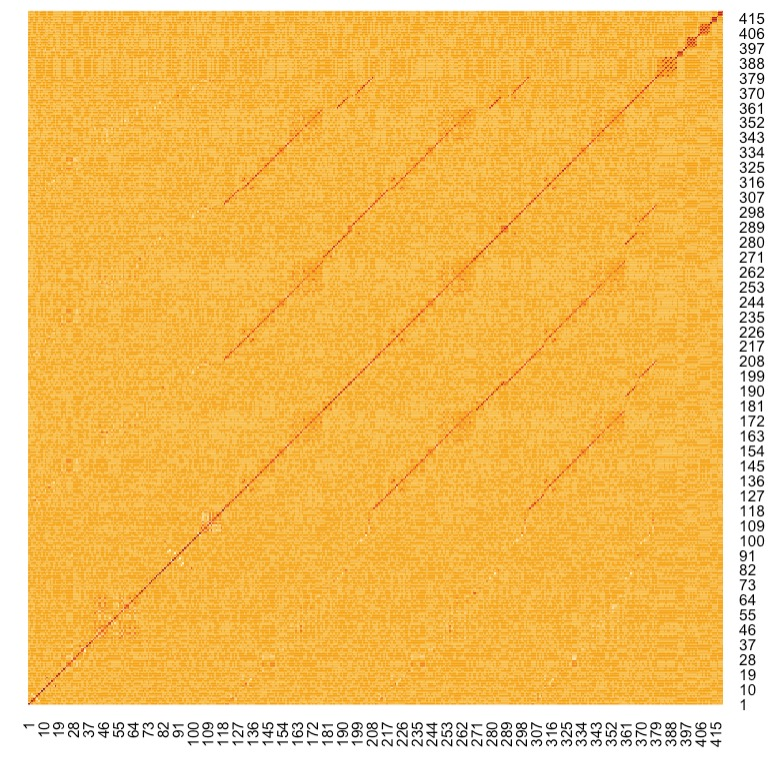
\includegraphics[height=6cm,width=6cm]{sigma1.jpg} 
    %\caption*{(a) Sample Covariance Matrix $\bm \Sigma$}
    \end{minipage} 
    \begin{minipage}[t]{0.5\linewidth}
    \centering 
    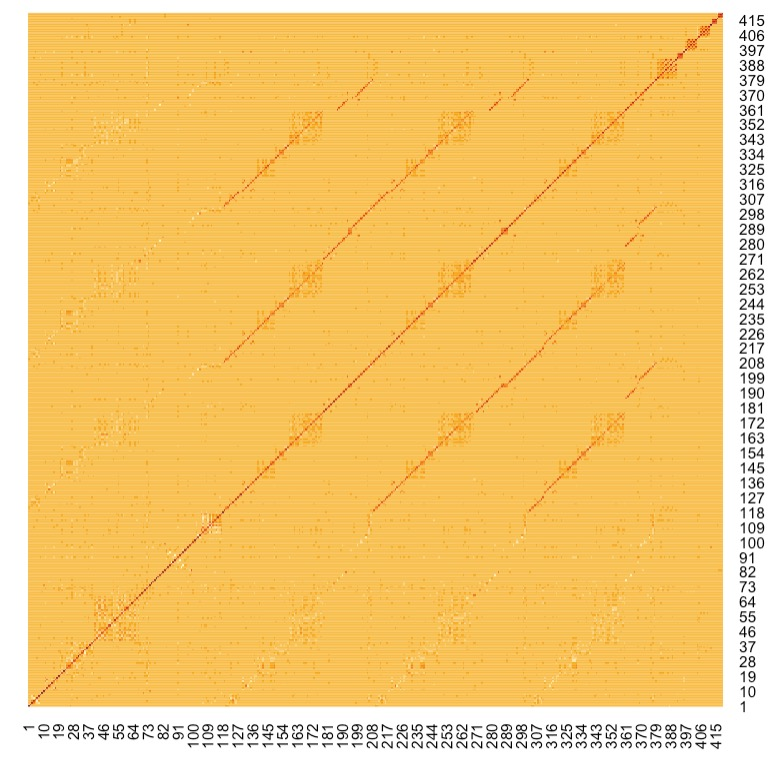
\includegraphics[height=6cm,width=6cm]{sigma2.jpg} 
    %\caption*{(b) Adjusted Covariance Matrix $ \hat{\bm \Sigma}$} 
    \end{minipage} 
    \caption{HeatMaps of the Correlation Structure of sample (Left) and adjusted (Right) covariance matrix of the transformed data streams}
    \label{cov}
\end{figure} 

\subsection{Fault diagnosis of the semiconductor manufacturing data}
We applied the top-r scheme in Section 3 with $r=25, 50, 75, 100$ on this dataset, and the threshold parameter $a$ was chosen such that the expected stopping time under the null hypothesis $H_0:\bm\mu=\bm{0}$ is around 400. From Table \ref{emp}, we can see that there is a great drop, from 51 to 36, in the stopping time for increasing $r$ from 25 to 50. It suggests that the number of OC data streams is much greater than 25, so that using only the top 25 data stream lose significant power for detecting mean shifts and hence the detection time is delayed. There is also a drop, from 36 to 28, when $r$ increase from 50 to 75, but essentially the same stopping time for $r=75$ and $r=100$. It suggests that there are more than 50 OC data streams, but no more than 75 significant data streams. 

As shown in Theorem 1, our knockoff procedure just need to be applied once in order to control the FDR. However, since there exits randomness in the knockoff procedure due to the knockoff copies generation, the rejection set of the knockoff procedure might change dynamically in each execution. To make the result of knockoff procedure more robust, we repeatedly executed the knockoff procedure 100 times and computed the rejection proportion of each data stream. Let $N_{rej}$ be the number of rejection in a knockoff procedure. We estimated the expectation $E(N_{rej})$ by the average of those 100 numbers of rejection in 100 knockoff procedures, and then rejected $H_j$ if the $j$th data stream has the top $E(N_{rej})$ largest rejection proportion. We considered the knockoff procedure with significant level 0.1. The expected stopping time $E(\tau^{KF})$ and the expected number of rejection of the knockoff procedures for various $r$ are shown in Table \ref{emp}, and the rejection proportions of the data streams that have proportion greater than 0.5 for some $r\in\{25,50,75,100\}$ are shown in Table \ref{tab:addlabel}. We observe that $E(\tau^{KF})$ are strictly less than $\tau^{obs}$. It is expected by the definition of $\tau^{KF}$. It is also not surprising that $E(\tau^{KF})$ are close to $\tau^{obs}$ as the knockoff copies were (approximately) generated under global null. The expected number of rejection decreases as $r$ increases. It is because there are more samples (longer stopping time) for smaller $r$. The results in Table \ref{emp} shows that there are 20 to 25 data streams giving strong signals of mean shift and there are some weaker signals require more samples to detect. This conclusion can be also seen in the rejection proportions in Table \ref{tab:addlabel}, which shows that almost all data streams having rejection proportion greater than 0.5 in the setting of $r=50,75$ or $100$ also have rejection proportion greater than 0.5. However, there are two exceptions, data streams V435 and V390, which essentially cannot be detected for the case $r=25$ but have high rejection proportions for other cases. To investigate the reason, we plotted the CUSUM statistics for these 2 data streams and indicated the statistics at expected stopping times $E(\tau^{KF})$ by blue circles. We found that the plots are flattened after the stopping time corresponding to $r=50$. However, if there is a positive mean shift, the plot of CUSUM statistics should show an increasing trend. The plots in Figure 2 suggest that the assumption of consistent mean shift may not hold for these two data streams.   


% Table generated by Excel2LaTeX from sheet 'Sheet1'
\begin{table}[htbp]
  \centering
  \caption{The observed stopping time of the top-$r$ scheme, the expected stopping time and the expected number of rejection of 100 knockoff procedures for various $r$. The values in parentheses are corresponding standard deviations.}
    \begin{tabular}{rcccc}
    \toprule
    r& a & $\tau^{obs}$ & $E(\tau^{KF})$ & $E(N_{rej})$ \\
        \midrule
    25 & 302 & 51 & 50.52(0.70) & 39.57(7.85) \\
    50 & 375 & 36 & 31.97(2.08) & 25.97(7.53) \\
    75 & 430 & 28 & 26.71(0.46) & 23.37(8.83) \\
    100 & 480 & 27 & 24.92(0.37) & 22.97(5.92) \\
        \bottomrule
    \end{tabular}%
  \label{emp}%
\end{table}%


\begin{table}[htbp]
  \centering
  \caption{Proportion of Rejection by Knockoff Procedure}
    \begin{tabular}{lrrrr}
    \toprule
    Stream \# & \multicolumn{1}{r}{r=25} & \multicolumn{1}{r}{r=50} & \multicolumn{1}{r}{r=75} & \multicolumn{1}{r}{r=100} \\
      \midrule
    V39 & 1 & 0.94 & 0.97 & 0.92 \\
    V60 & 1 & 1 & 0.98 & 0.99 \\
    V161 & 1 & 1 & 0.98 & 0.98 \\
    V551 & 1 & 1 & 0.98 & 0.99 \\
    V554 & 1 & 1 & 0.93 & 0.95 \\
    V557 & 1 & 1 & 0.98 & 0.99 \\
    V206 & 1 & 0.98 & 0.05 & 0.03 \\
    V104 & 1 & 0.97 & 0.76 & 0.84 \\
    V113 & 1 & 0.95 & 0.49 & 0.56 \\
    V342 & 1 & 0.95 & 0.22 & 0.29 \\
    V248 & 1 & 0.93 & 0.82 & 0.84 \\
    V296 & 1 & 0.49 & 0.98 & 0.99 \\
    V432 & 1 & 0.47 & 0.98 & 0.98 \\
    V214 & 1 & 0.01 & 0.08 & 0.18 \\
    V352 & 1 & 0.01 & 0.04 & 0.13 \\
    V288 & 1 & 0 & 0.01 & 0.06 \\
    V156 & 0.99 & 0 & 0 & 0 \\
    V511 & 0.99 & 0.99 & 0.92 & 0.82 \\
    V386 & 0.99 & 0.98 & 0.98 & 0.99 \\
    V520 & 0.99 & 0.86 & 0.6 & 0.62 \\
    V429 & 0.99 & 0 & 0 & 0 \\
    V291 & 0.98 & 0 & 0.04 & 0.11 \\
    V125 & 0.95 & 0.14 & 0.05 & 0.2 \\
    V478 & 0.93 & 0.66 & 0 & 0 \\
    V349 & 0.92 & 0.3 & 0.35 & 0.36 \\
    V80 & 0.89 & 0.09 & 0.04 & 0.02 \\
    V38 & 0.88 & 0.67 & 0.35 & 0.27 \\
    V130 & 0.8 & 0.02 & 0 & 0.01 \\
    V22 & 0.79 & 0.58 & 0.92 & 0.87 \\
    V299 & 0.76 & 0.97 & 0.89 & 0.98 \\
    V34 & 0.7 & 0.33 & 0.28 & 0.62 \\
    V164 & 0.67 & 0.95 & 0.85 & 0.93 \\
    V211 & 0.65 & 0.46 & 0.32 & 0.42 \\
    V37 & 0.52 & 0.02 & 0.01 & 0 \\
    V57 & 0.52 & 0.01 & 0 & 0 \\
    V369 & 0.52 & 0.6 & 0.32 & 0.19 \\
    V358 & 0.46 & 0.04 & 0.03 & 0.03 \\
    V176 & 0.45 & 0.3 & 0.05 & 0.08 \\
    V64 & 0.43 & 0 & 0.01 & 0.02 \\
    V426 & 0.41 & 0 & 0.01 & 0.02 \\
    V435 & 0.01 & 1 & 0.98 & 0.99 \\
    V390 & 0.05 & 0.77 & 0.68 & 0.86 \\
    V272 & 0.19 & 0.43 & 0.38 & 0.35 \\
    V56 & 0.1 & 0.35 & 0.5 & 0.49 \\
      \bottomrule
    \end{tabular}%
  \label{tab:addlabel}%
\end{table}%


\begin{figure}[H]
\centering
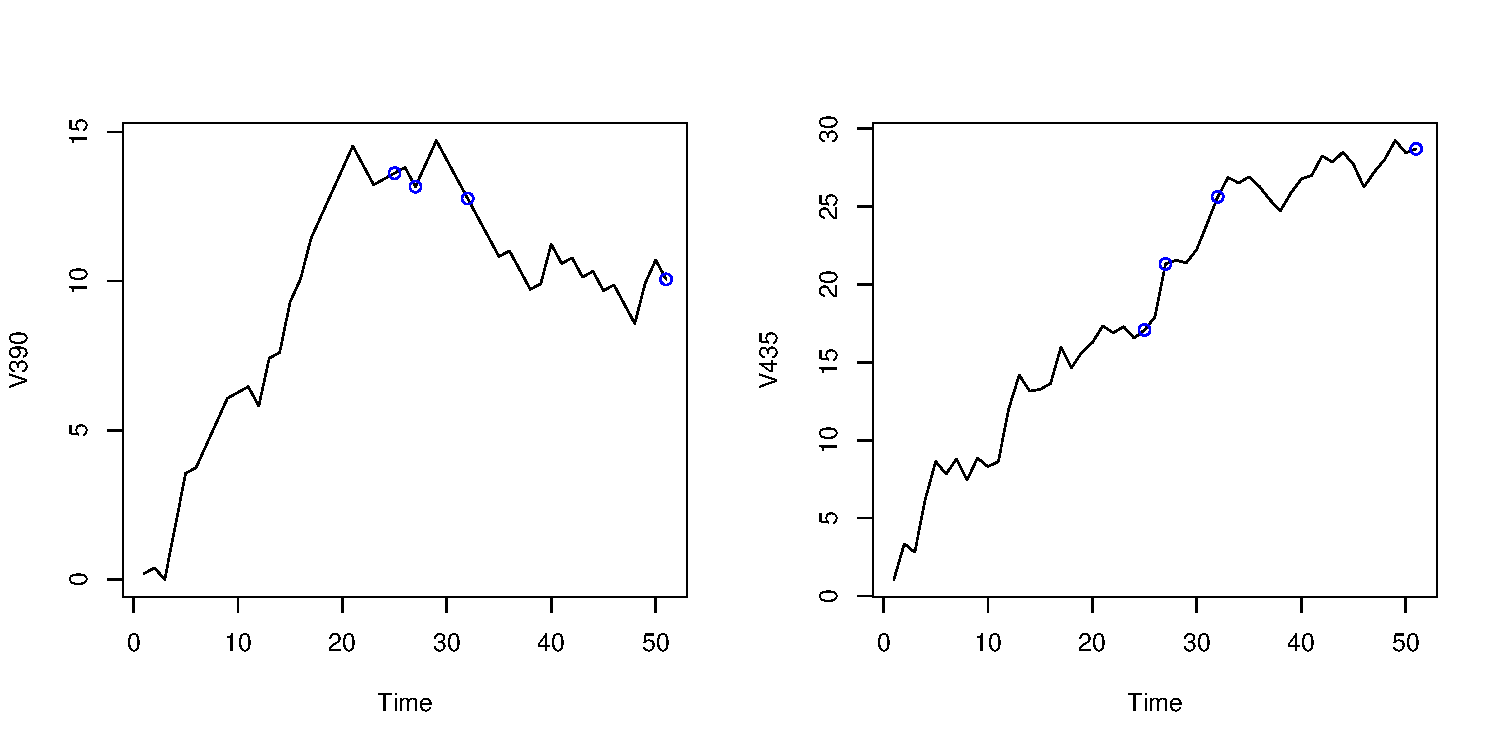
\includegraphics[scale=0.6]{390435}
\caption{CUSUM Statistics of Stream V390 and V435}
%\label{fig_V390V435}
\end{figure}


\section{Concluding remarks}

Although many methods have been proposed for fault detection and have been showed to have good performance in terms of giving signals quickly after the mean shift, they are not designed for fault identification and hence can perform very poor for controlling false discoveries, as we have seen in our simulations. Our proposed knockoff procedure apply the ideas of knockoff filtering proposed by \cite{barber2015controlling} to help those existing fault detection methods control FDR while maintain high power. Note that the knockoff procedure does not involve the fault detection part and hence the power of detection for the knockoff modified procedure is exactly the same as the original detection procedure. Another advantage of the proposed knockoff procedure is that it does not require additional samples after OC signals are detected for the control of FDR. As we have illustrated in the knockoff top-$r$ and knockoff FDR-adjusted Shewhart chart examples, we can ensure that the new stopping time $\tau^{KF}$ is smaller than the observed stopping time $\tau^{obs}$ and the new knockoff copies are generated based on the observed samples. It is an important property since it is usually the case that no more OC samples generated after an OC signal is detected.

The strength of the knockoff procedure is that it can control FDR in finite samples without any assumptions about the dependence among the data streams. Note that the common used BHq procedure requires the $p$-values are positively regression dependent, see \cite{benjamini2006adaptive}. However, it is not generally true in the multivariate SPC problems. For example, the $\mathbf{d}_{\cdot,t}$ in the  
example of FDR-adjusted Shewhart chart are not positively regression dependent. Although we assume normal distributions for the data streams $\mathbf{X}_t$, which is common assumed in the literature, algorithms for gnerating knockoff copies for general distributions have been recently introduced in \cite{BatesEtAl2020}.

%\clearpage







\appendix
\setcounter{equation}{0} 
\renewcommand{\theequation}{A\arabic{equation}}
\section{Proof of Theorem \ref{theo1}}
Let $S^+(t) = \{j: W_j \ge t\}, S^-(t) = \{j: W_j \ge -t\}$, then the selected set is $\hat S = S^+(t_{\min})$. Note that, by the construction of $W_j$, $P(W_j=0)=0$. Without loss of generality, we assume $|W_1| \ge |W_2| \ge \cdots \ge |W_p| > 0$, and then we can rewrite $\hat S = S^+\left (|W_{\hat k}|\right ) = \left \{ j \le \hat k: W_j >0\right \}$, where
$$
\hat k = \max \left \{k: \frac{1 + \left|S^-\left(\left|W_k\right|\right)\right|}{\max \{1, \left|S^+\left(\left|W_k\right|\right)\right|\}} \le \alpha \right \}.
$$
Note that $ \left|S^-\left(\left|W_{\hat k}\right|\right)\right| = \left \{ j \le \hat k: W_j < 0\right \}$ and hence
\begin{equation}\label{apeq1}
FDP = \frac{\# \{j \in H_0: j \in \left|S^+\left(\left|W_{\hat k}\right|\right)\right|\}}{\max \{1, \left|S^+\left(\left|W_{\hat k}\right|\right)\right|\}\}}  \le \alpha \frac{V^+(\hat k)}{1 + V^-(\hat k)}
\end{equation}
where $V^+(k) = \# \{j \in H_0: 1 \le j \le k, W_j > 0\}$ and $V^-(k) = \# \{j \in H_0: 1 \le j \le k, W_j < 0\}$. By the same argument of the proof Lemma 4 in \cite{barber2015controlling}, we have
\begin{equation}\label{apeq2}
\E \left(\frac{V^+(\hat k)}{1 + V^-(\hat k)}\right) \le\E \left(\frac{V^+(p)}{1 + V^-(p)}\right) =  \E \left(\frac{V^+}{1 + p_0 - V^+}\right).
\end{equation}
Since $V_0^+$ is stochastically greater than $V^+$, and $f(x) = x/(1+p_0-x)$ is nondecreasing, we have
\begin{equation}\label{apeq3}
\E \left(\frac{V^+}{1 + p_0 - V^+}\right) \le \E \left(\frac{V^+_0}{1 + p_0 - V^+_0} \right) \le 1.
\end{equation}
The last inequality comes from the proof Lemma 4 in \cite{barber2015controlling}. Combining (\ref{apeq1}), (\ref{apeq2}) and (\ref{apeq3}) yields the result in Theorem \ref{theo1}.


%\clearpage




%\section{References}

\bibliographystyle{apacite}
\bibliography{bibliography}


\end{document}